\chapter[Радиостанции]{Радиостанции}
\label{ch:radio-station}

Радиостанции — комплекс устройств и сооружений, служащих для подготовки программ радиовещания. Данная статья посвящена исследованию радиостанций на основе Викиданных. Для исследования спроектированы SPARQL-запросы, работающие с объектами Викиданных типа “radio stations”. Получен список всех радиостанций, описанных в Викиданных.

\marginnote{Используемые в запросах объекты: \wdqName {<<радиостанции>>}{Q14350};
Используемое свойство: \wdProperty{31}{<<экземпляр>>}}

\subsection{Список количества радиостанций}

\begin{lstlisting}
SELECT ?radioLabel ?countryLabel WHERE
{
    ?radio wdt:P31 wd:Q14350. # instance of radio station
    ?radio wdt:P495 ?country. # country of origin
    SERVICE wikibase:label { bd:serviceParam wikibase:language "ru,en,[AUTO_LANGUAGE]" }
}
\end{lstlisting}%

\footnotetext{Получено: \num{113} результатов на 2022 год. Ссылка на SPARQL-запрос: \href{https://w.wiki/5unA}{SPARQL-запрос}.}

\newpage

Посмотрим количество радиостанций у разных стран.

Количество радиостанций у разных стран.

\begin{lstlisting}
SELECT (COUNT(?radio) as ?sumRadio) ?countryLabel
WHERE {
  ?radio wdt:P31 wd:Q14350; # instance of radio station
         wdt:P495 ?country. # country of origin
  SERVICE wikibase:label { bd:serviceParam wikibase:language "ru,en,[AUTO_LANGUAGE]" }
}
GROUP BY ?countryLabel
ORDER BY DESC (?sumRadio)
\end{lstlisting}%

\footnotetext{Получено: \num{29} результатов на 2022 год. Ссылка на SPARQL-запрос: \href{https://w.wiki/62MJ}{SPARQL-запрос}.}

\begin{table}[ht]
\centering
\caption{Количество радиостанций по убыванию у 10 стран на 2022 год.}
\begin{tabular}{|c|c|c|}
\hline
Номер & Количество радиостанций по "country of origin" (P495) & Страна \\
\hline
1 & 15840 & США \\
2 & 1565 & Мексика \\
3 & 1299 & Канада \\
4 & 995 & Филиппины \\
5 & 800 & Великобритания \\
6 & 772 & Бразилия \\
7 & 571 & Германия \\
8 & 451 & Австралия \\
9 & 427 & Франция \\
10 & 370 & Индия \\
... & ... & ... \\
23 & 82 & Россия \\
... & ... & ... \\
32 & 51 & Нидерланды \\
\hline
\end{tabular}
\end{table}

Всего в мире около двухсот стран (смотри страницу Страны), но наш скрипт нашёл только \num{29} стран, в которых есть радиостанции. Поскольку радиостанции есть в каждой стране мира, то результаты скрипта говорят о неполноте Викиданных.

\newpage

Мы переделали скрипт, указанный выше, изменив в нём P495 (страна происхождения) на на P17 (государство).

\begin{lstlisting}
SELECT (COUNT(?radio) as ?sumRadio) ?countryLabel
WHERE {
  ?radio wdt:P31 wd:Q14350; # instance of radio station
         wdt:P17 ?country. # country of origin
  SERVICE wikibase:label { bd:serviceParam wikibase:language "ru,en,[AUTO_LANGUAGE]" }
}
GROUP BY ?countryLabel
ORDER BY DESC (?sumRadio)\end{lstlisting}%

\footnotetext{Получено: \num{196} результатов на 2022 год. Ссылка на SPARQL-запрос: \href{https://w.wiki/66bR}{SPARQL-запрос}. }

В итоге мы нашли \num{196} стран, имеющие радиостанции(таблица была изменена на основе нового кода).

Получим скрипт, который выводит спсиок подклассов радиостанций. Для каждого класса укажем число его экземпляров.

\begin{lstlisting}
SELECT ?subRadio ?subRadioLabel (COUNT(?r) AS ?count) WHERE
{
  ?subRadio wdt:P279* wd:Q14350. # subclass of radio station
  ?r wdt:P31 ?subRadio # instance of subclass of radio station 
  SERVICE wikibase:label { bd:serviceParam wikibase:language "ru,en" }
}
GROUP BY ?subRadio ?subRadioLabel
ORDER BY DESC(?count)\end{lstlisting}%

\footnotetext{Получено: \num{15} результатов на 2022 год. Ссылкаа на SPARQL-запрос: \href{https://w.wiki/62ML}{SPARQL-запрос}. }

\newpage

\subsection{Радиостанции, СМИ и вещательные каналы России}

Здесь представлен скрипт, который ведёт поиск радиостанций, вещательных каналов и СМИ по России, и по СССР без использования VALUES.

\begin{lstlisting}
SELECT ?radio ?radioLabel
WHERE
{
    {?radio wdt:P31 wd:Q14350.} UNION # instance of radio station
    {?radio wdt:P31 wd:Q15265344.} UNION # instance of broadcasting
    {?radio wdt:P31 wd:Q11033.} # instance of mass media
    
    {?radio wdt:P17 wd:Q159.} UNION # in Russia
    {?radio wdt:P17 wd:Q15180.} # in USSR
    SERVICE wikibase:label { bd:serviceParam wikibase:language "ru,en,[AUTO_LANGUAGE]". }
}\end{lstlisting}%

\footnotetext{Получено: \num{117} результатов на 2023 год. Ссылка на SPARQL-запрос: \href{https://w.wiki/6Lup}{SPARQL-запрос}. }

Расширен предыдущий скрипт, чтобы включить вещательные каналы и СМИ и сделать поиск и по России, и по СССР.

\begin{lstlisting}
SELECT  ?radio  ?radioLabel
WHERE
{
  {?radio wdt:P31 wd:Q14350.} UNION # instance of radio station
  {?radio wdt:P31 wd:Q15265344.} UNION # instance of broadcasting
  {?radio wdt:P31 wd:Q11033.} #instance of mass media
  
  # Soviet Union and Russia
  VALUES ?ruCountries {wd:Q15180 wd:Q159}
  ?radio wdt:P17 ?ruCountries. # related to Russian countries
  
  SERVICE wikibase:label {bd:serviceParam wikibase:language "ru,en"}
}\end{lstlisting}%

\footnotetext{Получено: \num{117} результатов на 2023 год. Ссылка на SPARQL-запрос: \href{https://w.wiki/6LU7}{SPARQL-запрос}. }

\newpage

\subsection{Тематика радиостанций России и СССР}

Данный скрипт предназначен для поиска тематик радиостанций, СМИ и вещательных каналов.

\begin{lstlisting}
SELECT ?radio ?radioName (GROUP_CONCAT(DISTINCT ?mainSubjectLabel;separator=", ") AS ?mainSubjects) 
WHERE
{
  {?radio wdt:P31 wd:Q14350.} UNION # instance of radio station
  {?radio wdt:P31 wd:Q15265344.} UNION # instance of broadcasting
  {?radio wdt:P31 wd:Q11033.} #instance of mass media
  
  # Soviet Union and Russia
  VALUES ?ruCountries {wd:Q15180 wd:Q159}
  ?radio wdt:P17 ?ruCountries. # related to Russian countries
  
  ?radio wdt:P921 ?mainSubject.
  
  SERVICE wikibase:label { bd:serviceParam wikibase:language "ru,en".
                         ?radio rdfs:label ?radioName .
                         ?mainSubject rdfs:label ?mainSubjectLabel .}
} GROUP BY ?radio ?radioName\end{lstlisting}%

\footnotetext{Получено: \num{74} результатов на 2023 год. Ссылка на SPARQL-запрос: \href{https://w.wiki/6b7P}{SPARQL-запрос}. }

\newpage

\begin{table}[ht]
\centering
\caption{Количество тематик у радиостанций, СМИ и вещательных каналов по убыванию на 2023 год}
\begin{tabular}{|c|c|}
\hline
Количество тематик по "main subject" (P921) & Название тематики \\
\hline
44 & музыка \\
30 & новости \\
15 & политика \\
9 & ток-шоу \\
7 & экономика \\
5 & спорт \\
5 & рок \\
5 & пропаганда \\
5 & проект \\
5 & поп-музыка \\
5 & авария \\
3 & TopHit \\
3 & шутка \\
3 & хип-хоп \\
3 & спектакль \\
3 & молодёжная музыка \\
3 & джаз \\
2 & юмор \\
2 & художественная литература \\
2 & комедия \\
2 & политическая система России \\
\hline
\end{tabular}
\end{table}

\newpage

В скрипте выше функция GROUP\_CONCAT объядиняет (конкатенация строк) содержимое меток (rdfs:label) главных тем (wdt:P921) радиостанций. Эта функция объединяет строки, вставляя между ними разделитель (по умолчанию разделитель -- запятая). В следующей таблице приведены пример конкатенации главныз тем для СМИ 7x7 и газеты <<Молодой дальевосточник>>.

\begin{table}[ht]
\centering
\caption{Пример использования функции GROUP\_CONCAT}
\begin{tabular}{|p{14em}|p{10em}|p{10em}|}
\hline
radio & radioName & mainSubject \\
\hline
wd:Q104538016 & [[w:7x7|7x7]] & экология, политика, новости, субъект Российской Федерации, правозащитник \\
\hline
[[d:Q30909585|wd:Q30909585]] & Общественно-политический еженедельник Молодой дальневосточник XXI век & война, спорт, экономика, реклама, новости, путешествие \\
\hline
\end{tabular}
\end{table}

\newpage

\subsection{Радиостанции, СМИ и вещательные каналы в социальных сетях}

Данный скрипт находит аккаунты радиостанций, СМИ и вещательных каналов в социальных сетях.

\begin{lstlisting}defaultView:BubbleChart
SELECT ?netID ?netIDLabel ?netRelation (COUNT(?network) as ?sumNetwork)
WHERE
{                  # Facebook, Instagram, Telegram, Twitter, VK, YouTube, Zen, SoundCloud, Google ID, Odnoklassniki, Rutube, Spotify
  VALUES ?netRelation {wdt:P2013 wdt:P2003 wdt:P3789 wdt:P2002 wdt:P3185 wdt:P2397 wdt:P8816 wdt:P3040 wdt:P2847 wdt:P5163 wdt:P10152 wdt:P5916}
  
  ?radio wdt:P31 wd:Q14350; # instance of radio station
         wdt:P17 wd:Q159;   # radio from Russia
         ?netRelation ?network. # has social network page

  ?netID wikibase:directClaim ?netRelation.
  
  SERVICE wikibase:label {bd:serviceParam wikibase:language "en"}
} GROUP BY ?netID ?netIDLabel ?netRelation 
ORDER BY DESC(?sumNetwork)\end{lstlisting}%

\footnotetext{Получено: \num{12} результатов на 2023 год. Ссылка на SPARQL-запрос: \href{https://w.wiki/6fKb}{SPARQL-запрос}. }

Объясним строку "?netID wikibase:directClaim ?netRelation" и необходимость использования предиката wikibase:directClaim.

Для этого нужно начать с объяснения того, что радиостанции соответствует объект и страница на Викиданных. На этой странице есть подраздел Идентификаторы (Identifiers). В этом подразделе перечислены, в том числе, социальные сети, в которых зарегистрирован объект (здесь радиостанция). Два следующих утверждених из запроса выше (на примере ВКонтакте, которому соответствует идентификатор-свойство P3185):

\begin{lstlisting}
# VALUES ?netRelation ... wdt:P3185
# ?radio ... ?netRelation ?network. \# has social network page
\end{lstlisting}

мы получаем ?netRaletion для каждой радиостанции, счетчик ?sumNetwork (здесь для ВКонтакте) увеличивается на один.

Проблема в том, что мы не можем получить имя ?netRelationLabel, поскольку конструкция "SERVICE wikibase" не работает для свойств, а только для объектов. Нам помогает свойство wikibase:directClaim, которое возвращает имя (?netID) по свойству (?netRelation).

\newpage

Пузырьковая диаграмма показывает количество аккаунтов СМИ и радиостанций в социальных сетях. То есть на рисунке показаны социальные сети, размер круга пропорционален количеству зарегистрированных в них аккаунтов СМИ и радиостанций.

Популярными социальными сетями среди радиостанций, СМИ и вещательных каналов на 2023 год стали: № 1 ВКонтакте — 28 аккаунтов; № 2 Instagram — 26 аккаунтов; № 3 Facebook — 25 аккаунтов; № 4 YouTube — 24 аккаунта; № 5 Twitter — 21 аккаунт; № 6 Telegram — 20 аккаунтов. Таким образом, самой популярной социальной сетью для СМИ стал ВКонтакте.

\index{График!Sunburst diagram}
\begin{marginfigure}[1\baselineskip]
{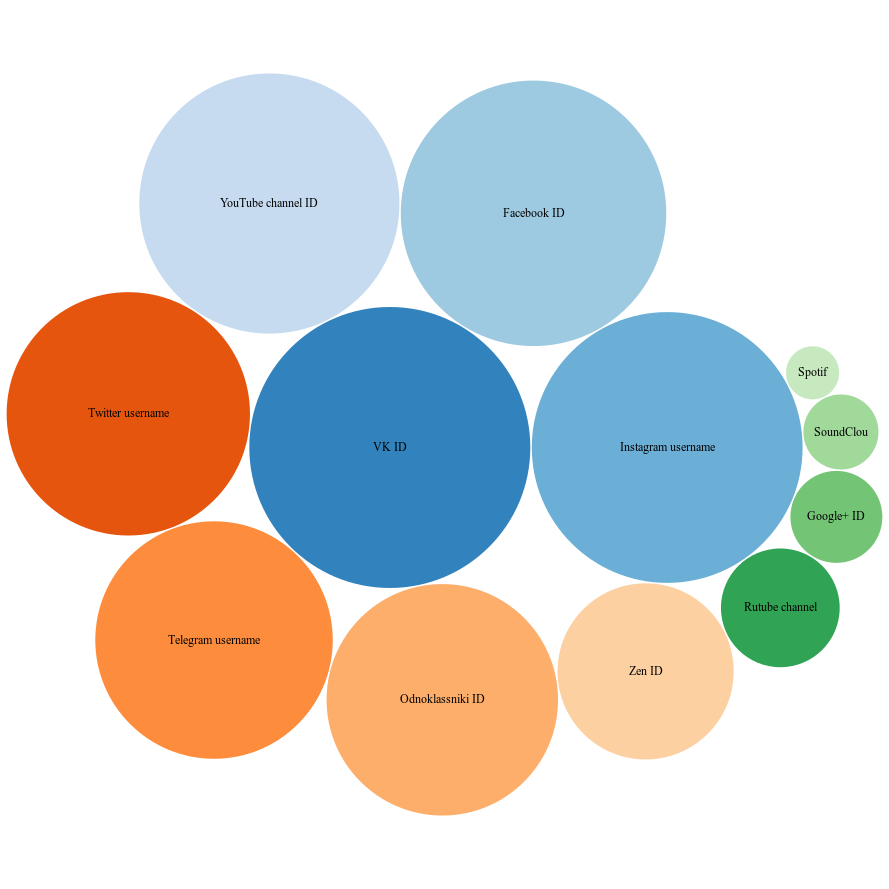
\includegraphics[width=1\linewidth]{chapter/radio_station/Number_of_social_media_accounts.png}}
\vspace{-7pt}
\caption{Аккаунты в социальных сетях}%
\label{fig:radio_station_acc}
\end{marginfigure}

%
